\section{Analisi dei costi}
L'analisi dei costi è stata effettuata impiegando un metodo di stima analitico,
poiché, essendo una proposta innovativa, non è stato possibile reperire dati
storici riguardanti i costi di progetti simili.
%%%%%%%%%%%%%%%%%%%%%%%%%%%%%%%%%%%%%%%%%%%%%%%%%%%%%%%%%%%%%%%%%%%%%%%%%%%%%%%%
%%%%%%%%%%%%%%%%%%%%%%%%%%%%%%%%%%%%%%%%%%%%%%%%%%%%%%%%%%%%%%%%%%%%%%%%%%%%%%%%
%%%%%%%%%%%%%%%%%%%%%%%%%%%%%%%%%%%%%%%%%%%%%%%%%%%%%%%%%%%%%%%%%%%%%%%%%%%%%%%%
%%%%%%%%%%%%%%%%%%%%%%%%%%%%%%%%%%%%%%%%%%%%%%%%%%%%%%%%%%%%%%%%%%%%%%%%%%%%%%%%
\subsection{Composizione del prodotto}
\subsubsection{Componenti hardware}
\begin{itemize}
\item \textbf{1 Arduino}: scheda elettronica dotata di microcontrollore per
attuare la logica di controllo dell’intero sistema
\item \textbf{4 Microcamere}: consentono la scansione delle immagini per il
riconoscimento delle api che ospitano il parassita
\item \textbf{Fotoresistore}: permette di tenere il conto delle api passate
sotto la microcamera, poiché questa non vede quelle senza varroa.
\item \textbf{1 Servomotore}: permette di indirizzare le api nell’arnia o nel
condotto di trattamento.
\item \textbf{1 Resistenza a cartuccia}: consente la sublimazione dell’acido
ossalico, è a base di nichel cromo, resistente all’ossidazione ed alla
corrosione.
\item \textbf{1 Sensore di temperatura}: consente il controllo della temperatura
del resistore
\item \textbf{1 Amplificatore di corrente}: fornisce la corrente di servizio
necessaria ai componenti elettrici
\item \textbf{1 Colorante gulal}: le api trattate vengono marcate in modo da non
venire ritrattate a breve termine
\item \textbf{1 Box contenitore}: struttura che contiene il prodotto
\end{itemize}
%%%%%%%%%%%%%%%%%%%%%%%%%%%%%%%%%%%%%%%%%%%%%%%%%%%%%%%%%%%%%%%%%%%%%%%%%%%%%%%%
%%%%%%%%%%%%%%%%%%%%%%%%%%%%%%%%%%%%%%%%%%%%%%%%%%%%%%%%%%%%%%%%%%%%%%%%%%%%%%%%
%%%%%%%%%%%%%%%%%%%%%%%%%%%%%%%%%%%%%%%%%%%%%%%%%%%%%%%%%%%%%%%%%%%%%%%%%%%%%%%%
%%%%%%%%%%%%%%%%%%%%%%%%%%%%%%%%%%%%%%%%%%%%%%%%%%%%%%%%%%%%%%%%%%%%%%%%%%%%%%%%
\subsubsection{Componenti software}
\begin{itemize}
\item \textbf{Programma di controllo}: Programma che pilota i dispositivi
hardware e descrive la logica di acquisizione dati, elaborazione ed attuazione
\end{itemize}
%%%%%%%%%%%%%%%%%%%%%%%%%%%%%%%%%%%%%%%%%%%%%%%%%%%%%%%%%%%%%%%%%%%%%%%%%%%%%%%%
%%%%%%%%%%%%%%%%%%%%%%%%%%%%%%%%%%%%%%%%%%%%%%%%%%%%%%%%%%%%%%%%%%%%%%%%%%%%%%%%
%%%%%%%%%%%%%%%%%%%%%%%%%%%%%%%%%%%%%%%%%%%%%%%%%%%%%%%%%%%%%%%%%%%%%%%%%%%%%%%%
%%%%%%%%%%%%%%%%%%%%%%%%%%%%%%%%%%%%%%%%%%%%%%%%%%%%%%%%%%%%%%%%%%%%%%%%%%%%%%%%
\subsection{Fasi di sviluppo del progetto}
\begin{itemize}
\item \textbf{Realizzazione del software}: questa fase raggruppa quelli che sono
i passaggi necessari per realizzare il prodotto software. In particolare, la
progettazione dell'architettura del software e lo sviluppo, il quale viene
commissionato a terzi.
\item \textbf{Inserimento in sede}: fase in cui viene selezionato e affittato
l'edificio in cui verranno assemblati i prodotti.
\item \textbf{Acquisto materie prime}: questa fase ricopre l'acquisto delle
componenti hardware.
\item \textbf{Assemblaggio materie prime e caricamento del software}.
\item \textbf{Vendita e spedizione del prodotto}.
\item \textbf{Assistenza}: fase in cui si offre servizio remoto di supporto.
\end{itemize}
%%%%%%%%%%%%%%%%%%%%%%%%%%%%%%%%%%%%%%%%%%%%%%%%%%%%%%%%%%%%%%%%%%%%%%%%%%%%%%%%
%%%%%%%%%%%%%%%%%%%%%%%%%%%%%%%%%%%%%%%%%%%%%%%%%%%%%%%%%%%%%%%%%%%%%%%%%%%%%%%%
%%%%%%%%%%%%%%%%%%%%%%%%%%%%%%%%%%%%%%%%%%%%%%%%%%%%%%%%%%%%%%%%%%%%%%%%%%%%%%%%
%%%%%%%%%%%%%%%%%%%%%%%%%%%%%%%%%%%%%%%%%%%%%%%%%%%%%%%%%%%%%%%%%%%%%%%%%%%%%%%%
\subsection{Stima delle risorse e dei costi}
Le risorse necessarie alla realizzazione del progetto vengono classificate e
quantificate seguendo una ripartizione tale da individuare costi fissi e
variabili.  
%
\subsubsection{Costi fissi}
I costi fissi sono tutti quei costi che non variano a seconda della domanda.

I costi sono stati classificati in “diretti” e “indiretti”. I costi diretti
riguardano le risorse umane o materiali necessarie esclusivamente alla
realizzazione del prodotto (materie prime, manodopera diretta, acquisto di beni
e servizi da terzi). I costi indiretti sono legati a manutenzione, ammortamenti,
energia e costi generali.\\
%
Sono stati individuati i seguenti costi fissi diretti:
\begin{itemize}
\item \textbf{Programmatori (\EUR{4000})}: risorse umane necessarie alla
realizzazione del software.  Le funzionalità del software riguardano
principalmente acquisizione dei dati, l’elaborazione, ed il controllo dei
dispositivi connessi alla scheda Arduino.  Per quanto riguarda l’acquisizione
dei dati tramite riconoscimento immagini, è già disponibile una libreria
software open source (OpenCV~\cite{opencv}) integrabile con la scheda, pertanto
si può considerare soltanto il costo di adattamento della libreria. Anche per
quanto riguarda le funzioni di controllo e attuazione, vi è un elevato grado di
supporto in casa Arduino, pertanto si stima un tempo necessario per
l’implementazione ed il test dell’ordine delle settimane, non più di 4, pari a
160 ore di lavoro. La retribuzione media per uno sviluppatore software in Italia
è stimata intorno ai 25 \EUR{} lordi (Job Pricing~\cite{corcom}), si può
concludere quindi che il costo totale sia al più di \EUR{4000} per un impiego
su commissione. 
\item \textbf{Computer (\EUR{1080})}: risorse materiali
necessarie per la gestione degli aspetti commerciali, contabilità, fatturazione
ed assistenza. Si prevede l’acquisto di 2 unità workstation per un costo di
\EUR{540} a macchina (Dell OptiPlex 3060 e monitor \cite{dell}).  
\item \textbf{Dipendenti (\EUR{4000}/mese)}: risorse umane con competenze
tecniche atte allo svolgimento delle mansioni necessarie all’attività
dell’azienda. Si prevede un impiego fisso per 8 ore al giorno per un totale di
\EUR{2000} lordi mensili per dipendente, in accordo con la stima relativa alle
retribuzioni medie di un impiegato in Italia secondo Job Pricing \cite{money}.
\end{itemize}
%
I costi fissi indiretti sono: 
\begin{itemize}
\item \textbf{Affitto immobile (\EUR{1000}/mese)}: locale di $100$ $m^2$
comprendente un magazzino per la giacenza dei prodotti e delle materie
prime, laboratorio di produzione, ufficio e bagno;
\item \textbf{Energia elettrica (\EUR{30}/mese)}: il consumo di energia è
legato all’illuminazione, all’utilizzo dei pc e al riscaldamento. Tramite
l’impiego di uno strumento online~\cite{lucegas} se ne è stimato il consumo
medio. Supponendo di avere un contatore di 3 kW (visto i pochi dispositivi
elettrici presenti e il basso numero di personale) e che l’immobile sia fornito
di una caldaia a condensazione, la stima risultante equivale a circa 1800
kWh/anno, cioè 150 kWh/mese. Per il primo trimestre del 2019 il prezzo del kWh è
di 0.2\euro/kWh~\cite{segugio} (comprendente materia prima, spese e tasse);

\item \textbf{Acqua (\EUR{10}/mese)}  è utilizzata solo per i servizi igienici.
Poiché una famiglia italiana consuma mediamente $200$ $m^3$ di acqua all’anno
\cite{acqua}, di cui la maggior parte è legata ad usi non-alimentari, sembra
ragionevole stimare di avere un consumo medio non superiore a $80$ $m^3$ di acqua
all’anno, per un costo mensile di \EUR{10} al mese (\EUR{1.37} per $m^3$
\cite{acquacub});

\item \textbf{Telefono (\EUR{35}/mese)} Costo per un abbonamento flat \cite{tim}
con chiamate illimitate e Internet.

\end{itemize}
%

L’ammontare totale dei costi fissi $\Phi$ è dato dalla somma delle spese mensili
ricorrenti:
\begin{displaymath}
\Phi = (4000 + 1000 + 30 + 10 + 35) \ \mbox{\euro/mese} = 5075 \ 
\mbox{\euro/mese}
\end{displaymath}
Nel calcolo non sono stati inseriti il costo dei computer e del software in
quanto non sono spese mensili ma effettuate solo all’inizio dell’attività.
Saranno ammortizzate nel bilancio annuale secondo le norme vigenti in Italia.
%
\subsubsection{Costi variabili}
I costi variabili sono invece tutti quei costi che variano a seconda della
domanda e quindi del volume di produzione.

La società dovrà acquistare i sensori per il monitoraggio dell’arnia e le
componenti per la somministrazione della cura alle api. Inoltre si aggiungono al
conto le spese di spedizione, in quanto il prodotto viene inviato al cliente che
provvede da solo all’installazione.\\
%
Di seguito i costi~\cite{hw} per componente elementare:
\begin{itemize}
\item \textbf{Arduino: \EUR{35}}
\item \textbf{Microcamere: \EUR{39.6}} ($4 \cdot 9.90$\EUR{})
\item \textbf{Fotoresistore: \EUR{1.50}}
\item \textbf{Servomotore: \EUR{3.20}}
\item \textbf{Resistenza: \EUR{12.00}}
\item \textbf{Sensore di temperatura: \EUR{2.00}}
\item \textbf{Amplificatore di corrente: \EUR{3.00}}
\item \textbf{Colorante: \EUR{13.00}}
\item \textbf{Box: \EUR{20.00}}
\item \textbf{Spese di trasporto: \EUR{16}} (prezzo medio per spedire in tutta
Italia un pacco del peso di circa 5 Kg)
\end{itemize}
L’ammontare dei costi variabili $\mu$ è
\begin{displaymath}
\mu= (35 + 39.6 + 1.5 + 3.2 + 12 + 2 + 3 + 13  + 20 + 16) \ \mbox{\euro} = 145.3
\ \mbox{\euro}
\end{displaymath}
Il costo finale per la produzione di un singolo prodotto è di $\mu$ = \EUR{145.3}.
%%%%%%%%%%%%%%%%%%%%%%%%%%%%%%%%%%%%%%%%%%%%%%%%%%%%%%%%%%%%%%%%%%%%%%%%%%%%%%%%
%%%%%%%%%%%%%%%%%%%%%%%%%%%%%%%%%%%%%%%%%%%%%%%%%%%%%%%%%%%%%%%%%%%%%%%%%%%%%%%%
%%%%%%%%%%%%%%%%%%%%%%%%%%%%%%%%%%%%%%%%%%%%%%%%%%%%%%%%%%%%%%%%%%%%%%%%%%%%%%%%
%%%%%%%%%%%%%%%%%%%%%%%%%%%%%%%%%%%%%%%%%%%%%%%%%%%%%%%%%%%%%%%%%%%%%%%%%%%%%%%%
\subsection{Ripartizione dei costi}
I costi definiti sono stati ripartiti in CAPEX e OPEX.\\
Il CAPEX (CAPital EXpenditure) rappresenta il costo per acquisire o sviluppare
asset durevoli per la società. Sono interpretati come capex per esempio i costi
relativi allo sviluppo software o l’affitto dei terminali.\\
L’OPEX (OPerating EXpense) rappresenta invece i costi operativi e di gestione
dell’azienda.

La classificazione dei costi è stata rappresentata nella tabella~\ref{tab:pex}.
Per la parte di costi OPEX riferiti al singolo prodotto si è proceduto a
calcolarli in relazione del numero stimato di clienti, in modo da poterne
definire il peso effettivo anno per anno, tale conto viene presentato nella
sezione \ref{sec:domanda} in cui si effettua l'analisi della domanda. 
Per quanto riguarda i costi CAPEX si è ottenuto un valore complessivo di
\EUR{5080}.

%tabella pex
\begin{table}[!h]
\centering
%\begin{adjustbox}{width=\textwidth}
\begin{tabular}{r@{\qquad}l|r@{\qquad}r}
 \multicolumn{2}{c}{CAPEX [\euro]}
& \multicolumn{2}{|c}{OPEX [\euro]/anno}
\\          
\hline
 Computer    & 1080  & Componenti HW (per prodotto) & 96.3 \\
 Sviluppo SW & 4000  & Spedizione    (per prodotto) & 16   \\ 
             &       & Box           (per prodotto) & 20   \\
             &       & Colorante     (per prodotto) & 13   \\
             &       & Utenze           & 900  \\
             &       & Stipendi         & 48000  \\
             &       & Affitto immobile & 12000  \\
\end{tabular}
%\end{adjustbox}
\caption{CAPEX \& OPEX}
\label{tab:pex}
\end{table}



Si è stimato dai costi trovati che 6 mesi di attività costeranno all’azienda
circa \EUR{79120}, quindi si è previsto un investimento iniziale di \EUR{80000}
composto per il 60\% da capitale proprio e per il 40\% da capitale ottenuto
tramite finanziamento da un istituto di credito.
%%%%%%%%%%%%%%%%%%%%%%%%%%%%%%%%%%%%%%%%%%%%%%%%%%%%%%%%%%%%%%%%%%%%%%%%%%%%%%%%
%%%%%%%%%%%%%%%%%%%%%%%%%%%%%%%%%%%%%%%%%%%%%%%%%%%%%%%%%%%%%%%%%%%%%%%%%%%%%%%%
%%%%%%%%%%%%%%%%%%%%%%%%%%%%%%%%%%%%%%%%%%%%%%%%%%%%%%%%%%%%%%%%%%%%%%%%%%%%%%%%
%%%%%%%%%%%%%%%%%%%%%%%%%%%%%%%%%%%%%%%%%%%%%%%%%%%%%%%%%%%%%%%%%%%%%%%%%%%%%%%%
\subsection{Determinazione del prezzo}
Non essendo ancora in possesso di dati sperimentali sulla risposta della domanda
in funzione del prezzo, si è ipotizzata una relazione descritta da funzione di
potenza del tipo: 
\begin{displaymath}
q = \alpha p^{-\beta}
\end{displaymath}
dove $\beta$ corrisponde all’elasticità della domanda.\\
Considerando una reazione significativa del consumatore al variare del prezzo
dovuta al fatto che si è un’azienda appena nata, si è supposto di avere una
domanda elastica ($\beta > 1$), quindi il prezzo ottimo sarebbe idealmente il
prezzo più basso possibile relativamente a quello imposto dalla concorrenza.
Il prezzo finale è stato determinato tenendo in considerazione i prezzi dei
prodotti più simili a \textit{BeeCareful} in termini di componenti hardware, che
identificano la fascia di prezzo compresa tra i \EUR{300} e i \EUR{500},
differenziandosi dai prodotti più costosi che permettono la raccolta dati
e l’accesso remoto agli stessi.

Per poter essere competitivi in un mercato così frammentato, abbiamo deciso di
fissare il prezzo di vendita a \EUR{350}, leggermente al di sopra del prezzo
ottimo poiché il prodotto una soluzione ad un problema che non viene risolto
dalla concorrenza.
%%%%%%%%%%%%%%%%%%%%%%%%%%%%%%%%%%%%%%%%%%%%%%%%%%%%%%%%%%%%%%%%%%%%%%%%%%%%%%%%
%%%%%%%%%%%%%%%%%%%%%%%%%%%%%%%%%%%%%%%%%%%%%%%%%%%%%%%%%%%%%%%%%%%%%%%%%%%%%%%%
%%%%%%%%%%%%%%%%%%%%%%%%%%%%%%%%%%%%%%%%%%%%%%%%%%%%%%%%%%%%%%%%%%%%%%%%%%%%%%%%
%%%%%%%%%%%%%%%%%%%%%%%%%%%%%%%%%%%%%%%%%%%%%%%%%%%%%%%%%%%%%%%%%%%%%%%%%%%%%%%%
\subsection{Break even point}
L’analisi del “punto di pareggio” è stata eseguita per determinare il volume di
produzione necessario per coprire i costi di produzione del prodotto.  Il punto
di break-even $q^*$ è dato dall’intersezione tra la retta dei costi e quella dei
ricavi. 
%
\setlength\arraycolsep{2pt}
\begin{displaymath}
\left\{ \begin{array}{rl}
c &= \phi + \mu q \\
r &= q p^* 
\end{array} \right .
\end{displaymath}
%
\begin{eqnarray*}
\phi &=& 5075 \cdot 12 = 60900 \ \mbox{\euro/anno} \qquad \mbox{costi fissi annuali} \\
p^* &=& 350 \ \mbox{\euro/prodotto} \ \qquad\quad\qquad\quad \mbox{prezzo
unitario} \\
\mu &=& 145.3 \ \mbox{\euro/prodotto} \ \qquad\quad\qquad\quad \mbox{costo variabile unitario}
\end{eqnarray*}
%
\begin{displaymath}
q^* = \frac{\phi}{p^* - \mu} = \frac{60900}{350 - 145.3} = 297.51 
\end{displaymath}
Quindi la vendita del duecentonovantottesimo prodotto ci permetterà di
arrivare al “punto di pareggio” tra costi e ricavi, mostrato in
figura~\ref{bep}, oltre tale soglia di vendita si avrà un guadagno positivo.
%
\begin{figure}[!h]
\centering
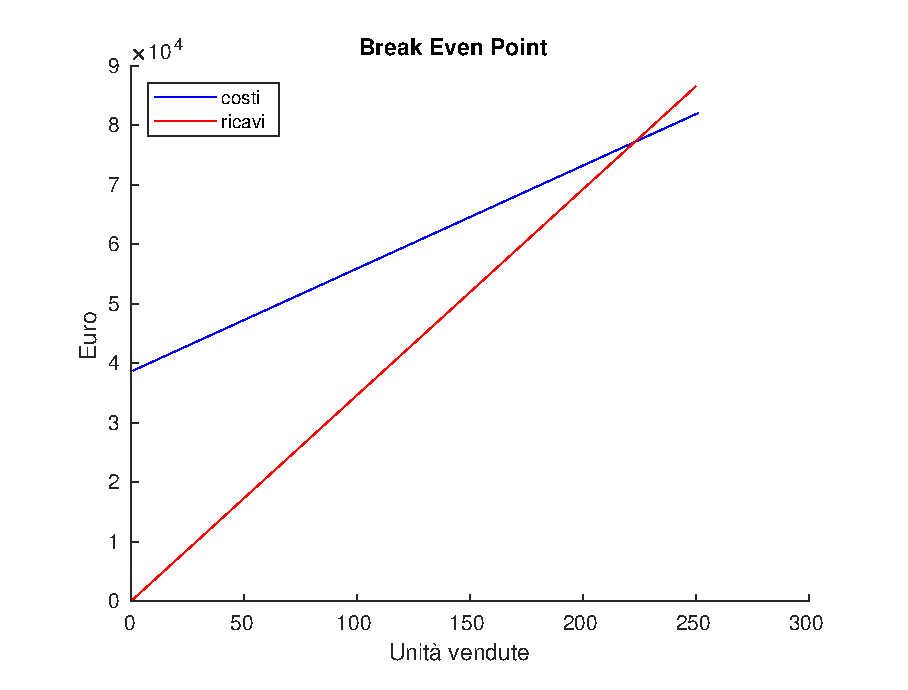
\includegraphics[width=\textwidth]{figures/bep}
\caption{Intersezione rette Costi e Ricavi}
\label{bep}
\end{figure}
%
